%%% Time-stamp: <2024-03-07 13:43:18 vladimir>
%%% Copyright (C) 2019-2024 Vladimir G. Ivanović
%%% Author: Vladimir G. Ivanović <vladimir@acm.org>
%%% ORCID: https://orcid.org/0000-0002-7802-7970

\chapter{Discussion}\label{ch:discussion}\indent%

This dissertation's research question (p.~\pageref{sec:research-question}): ``Has Rocketship structured itself to earn a return for its founders and investors, focusing especially on its real estate transactions?'' This question can be parsed into three sub-questions:
\begin{enumerate}
  \item Has Rocketship structured itself to make a profit?\footnote{Public benefit corporations (non-profits) are allowed to make a profit, i.e.\ revenue exceeds expenses; they are, however, not allowed to \textit{distribute} that profit. Any profit must be use to further is public benefit purpose identified in their articles of incorporation.}
  \item If so, is real estate the vehicle that Rocketship uses to make money?
  \item Is this Rocketship's intent?
\end{enumerate}

\index{key findings|(}%
After a careful examination of Rocketship's finances, it appears that Rocketship has, in fact, deliberately structured itself to make a profit using real estate as the means of generating that profit. However, a key finding is that the analysis of Rocketship's \textit{publicly available} financial documents show that any profits derived from operations of the schools appear to have been legally obtained and there is no evidence that these profits have been distributed to private persons, at least in California. But since some portion of these profits have been used to open non-profit charter schools in other states, no definitive finding can be made about the ultimate beneficiaries of these funds without further investigation. Some questionable expenditures were identified, namely \$7.5M spent on travel in 2019–2022. This is a large sum, and should also be investigated.%
\index{key findings|)}

The absence of evidence of illegal activity by Rocketship is fortunate because California is notorious for charter school fraud. In 2015, three advocacy organizations found \$81M in fraud \citeauthor{CPD2015.etal}. The report, \citetitle{CPD2015.etal} estimated in 2015 that, ``The vast majority of this fraud perpetuated by charter officials will go undetected because California lacks the oversight necessary to identify the fraud.'' \parencite[2]{CPD2015.etal}. A massive fraud was, fortunately, discovered in 2019: A single online charter school had defrauded the State of California of \$400M. With tens billions of dollars of funding for charter schools in California alone coupled with lax oversight, the temptation for fraud must be great. 

The next section presents an answer to this dissertation's research question. How that will be done is based on work done by Stephen Toulmin, a British philosopher interested in moral reasoning \parencite{Toulmin2003}. He developed in \citetitle{Toulmin2003} a method for making practical arguments where ethics and morality played a role. Toulmin arguments have been widely adopted. %chktex 12

\section{Answering the Research Question}\label{sec:answ-rese-quest}\indent

This dissertation's claim and conclusion is that Rocketship is structured and operates to leverage government funding (loans, grants, credit repair) which increases their real estate holdings, and this in turn allows them to open more charter schools. It does not appear that Rocketship is distributing profits to private parties such as its founders or investors.\label{p:claim}

This claim is the result of an extensive analysis of Rocketship's financial documents and board meeting packets. These show the extent to which Rocketship's leadership focuses, not on the academic success of its students, but rather on making sure that every Rocketship school is profitable. Rocketship's current assets, i.e. assets readily convertible into cash, have steadily increased from nearly \$9M in 2010 to over \$90M in 2022. This is a sizable war chest.

Right from the beginning, Rocketship's founders separated the financing, acquisition, and operation of their facilities from the pedagogical side of running a school. The founders borrowed heavily and made extensive use of government programs to fund their real estate projects. Rocketship's Santa Clara schools have not used alternative ways of acquiring facilities. They have not used Proposition 39 to obtain classrooms and fields from a school's home district. They have not tried to convert commercial office space into classrooms. They have not modified existing buildings to serve as schools or classrooms. Instead they bought land and built schools.

Rocketship’s policy of owning its facilities has led it to accumulate over \$185M of debt as of 2022, which comes to roughly \$32K per child. If that debt costs 3\% yearly to service, that is another \$5.4M per year that is not going directly toward educating children. Rocketship could have rented facilities with the rent being three quarters covered by SB 740 funds. In fact, the State of California does cover three quarters of the rent, but that rent goes to pay off loans taken out to purchase property owned by Launchpad Development. 

This focus on real estate shows up in the topics that the Rocketship Board and subcommittees discuss in meetings. Overwhelmingly, Rocketship's leaders and administrators met to discuss finance and real estate rather than curriculum or student achievement. An examination of the board meeting agendas for the first three years (2006–2009) show that no more than one out of five discussion topics concerned curriculum or student achievement. Judging just by the name of the board documents for the years 2020–2022, only 12 out of 108 (\approx11\%) were achievement related. Of the four board subcommittees (Achievement, Business, Executive, Development) three are focused on something other than student success.

Since Rocketship Education and Launchpad Development, as non-profit public benefit corporations, cannot distribute their income or assets to individuals or to for profit entities according to California law, IRS Code, and their Articles of Incorporation, Rocketship's leadership  likely had a different goal than enriching individuals. Rocketship Education's Amended and Restated Articles of Incorporation (2022) contains language that prohibits private enrichment. The language below taken directly from \textcite{RSED2022}, clearly prohibits private enrichment.
\begin{itemize}
  \item Article II. PURPOSE\\\noindent ``A. [Rocketship Education] is a nonprofit public benefit corporation'' ``not organized for the private gain of any person.''
  \item Article III. TAX-EXEMPT STATUS\\\noindent ``B. No part of the net earnings of this corporation shall inure to the benefit of, or be distributable to, any officer, director, or other private person, except that this corporation shall be authorized and empowered to pay reasonable compensation for services rendered and to make distributions in furtherance of its exempt purposes.''
  \item Article IV. IRREVOVABLE DEDICATION OF PROPERTY\\\noindent ``A. The property of this corporation is irrevocably dedicated to charitable purposes'' ``and no part of the net income or assets of this corporation shall ever inure to the benefit of any director, officer, or member thereof or to the benefit of any private person.''\\\noindent
  ``B. Upon dissolution or winding up of this corporation … its remaining assets shall be distributed to a nonprofit fund, foundation, association or corporation that is organized and operated exclusively for charitable purposes ….''
\end{itemize}

A possible objection is that the grounds given are neither necessary nor sufficient to prove the claim made on p.~\pageref{p:claim}; there could be reasons other than expansionary reasons for Rocketship to have structured themselves they way they did. True, and also true, is that the way they spend their time and money could have been forced on them by circumstance or by law. Also true.

As a rebuttal to these objections, both overlook the element of choice that Rocketship's leaders had when structuring their organization. The founders knew what they were getting themselves into because their board of directors and founders had both extensive real estate experience and charter school startup experience. They chose an organization that made RSED the decision maker and Launchpad the accumulator of value. They also understood that California law and IRS regulations didn't allow private enrichment because that was stated in their Articles of Incorporation. And lastly, they chose the purview of each board subcommittee. In other words, they were intentional in their choices because they had alternatives.

Rocketship's leadership could have chosen to make RSED (the parent organization) a 509(a)(3) supporting charity for individual 503(c)(3) non-profit public benefit corporations (the schools) and only provide requested services instead of forced management. Another alternative is that they could have even done away with RSED completely and just had a loose collection of independent charter schools. 

Rocketship had the freedom to choose their organizational structure. That combined with their knowledge that private enrichment is not allowed for non-profits, plus operating a sweep and having three times as many committees concerned with finances and real estate than on student outcomes strongly suggests that Rocketship founders and executives were strategic in their planning to prioritize real estate expansion. An early report, \citetitle{Carlisle.Kovalkoski2012} in 2012 states that ``The organization’s long-term goal is to expand from its seven existing schools to 2,000 schools in 50 cities, serving 1 million students.'' \parencite[3]{Carlisle.Kovalkoski2012}.

It is not publicly known why Rocketship's leadership has accumulated tens of millions of dollars in assets, nor is it known how they might convert those assets into transferable wealth. Perhaps they do not intend to do so. \prettyref{tab:types_conversion} below lists some of the forms and restrictions on converting real estate assets owned by a non-profit charter school.

\index{conversion, types of|(}
\noindent%
\begin{table}[htp]
  \caption[Types of Conversion]{\textit{Types of Conversion}}%
  \label{tab:types_conversion}
  \begin{tabulary}{0.9\textwidth}{LLL}
    \toprule
    \textbf{Type of Conversion} & \mbox{\textbf{Allowed?}} & \textbf{Notes} \\
    \midrule
    Excessive salaries & No & Listed in Form 990. Monitored by the IRS \vspace{6pt} \\
    Sale of assets to a private entity or for-profit corporation & No & Prohibited by CA Government Code, IRS Code, Articles of Incorporation. Requires AG notification \vspace{6pt} \\
    Sale of assets to another non-profit & Yes & Provided the non-profit has similar public benefit objectives \vspace{6pt} \\
    Conversion of property to condos or apts. & No & Non-profits restricted to charitable purposes \\
    \bottomrule
  \end{tabulary}
\end{table}
\index{conversion, types of|)}

\index{non-profit!private gain|(}
That then begs the question of why Rocketship is accumulating assets. According to California law and to IRS Code, charter schools are not allowed to transfer money to a for-profit entity or to private individuals. The option which makes the most sense in explaining Rocketship's structure and activities given the investments of Reed Hastings, Andre Agassi, the Walton Family Foundation, and others, all strong charter school supporters, is that Rocketship wants to become a self-perpetuating pipeline of new charter schools for the entire United States. Their expansion into Washington, D.C., Texas, Tennessee, and Wisconsin exactly fits this conjecture.

Another possibility for how Rocketship could dispose of its assets if and when all of its schools close is by transferring them to another non-profit, public benefit corporation.\footnote{It is unclear if transferring assets to a \textit{foreign} non-profit is permitted.} There are restrictions. The \citeauthor{CALDOJ2014} states in \textcite{CALDOJ2014} ``Any transfer of remaining assets inconsistent with the organization’s stated purpose may be subject to objections by the Attorney General.'' The stated purposes of Rocketship Education, Inc. in their \citetitle{RSED2022} are ``\ldots~to manage, operate, guide, direct and promote one or more public charter or other schools, other educational or community programs, and other charitable purposes.'' \parencite[1]{RSED2022}. This last clause opens the possibility that Rocketship at dissolution could donate all of its assets to any non-profit public benefit corporation, such as an affordable housing project. Since funding affordable housing and related services is critical in solving the problem of long-term housing for the homeless, keeping track of who funds these projects and how they are funded should be pursued, particularly when a particular housing project has both below market rate and market rate units.

It is also possible that the billionaires identified above have promised the founders or directors of Rocketship a bonus if they successfully create a model for self-perpetuating charter schools. Detecting such a payout, in another state or country would be difficult and would become increasingly difficult the longer the time lag between leaving Rocketship and receiving the payout. Tens of millions of dollars of bonus would not even rise to the level of a rounding error in the books of billionaires.
\index{non-profit!private gain|)}

\section{Public Policy Issues}%
\label{sec:publ-policy-chang}\indent%

\index{public policy issues|(}
There are at least three major public policy issues that are raised by Rocketship's growth in assets and presumed expansion goals. First, are charter schools or charter school chains a net benefit to Californians? Secondly, is there too much opportunity for fraud, and lastly, should charter school chains in California use their assets (paid for by Californians) to create charter schools in other states? This last public policy issue could be more broadly construed to ask if any Californian tax dollars should leave the state with no benefit to Californians.

The first of these public policy issues, the net benefit of Californian charter schools to California, is beyond the scope of this dissertation because it would require a thorough analysis of not only the finances of charter schools, but also of the costs and benefits of the education they offer, their impact on public schools, and their impact on the communities they serve. The second and third issues—opportunities for fraud and creating charter schools in other states—are discussed in the sections below.
\index{public policy issues|(}

\subsection{Fraud}%
\label{sec:fraud}\indent%

\index{public policy issues!fraud|(}
The Association of Certified Fraud Examiners issues an annual \textit{A Report to the Nations} which is a global study on occupational fraud. Of interest is a diagram of the types of occupational fraud, reproduced below.
\begin{figure}[htp]
  \caption{\textit{The Fraud Tree}}%
  \label{fig:fraud-tree}\centering%
  \copyrightbox[b] {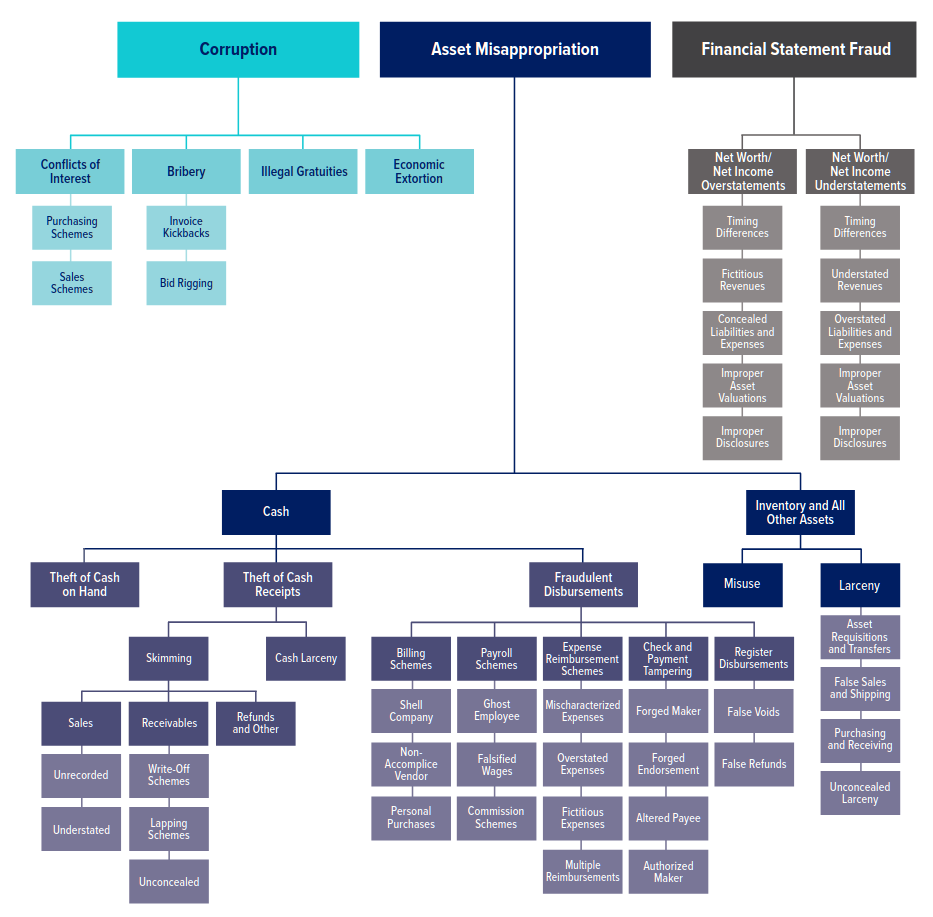
\includegraphics[width=0.85\textwidth]{2022 Report to the Nations-p.10}}
  {Reproduced by permission with attribution: \textit{Occupational Fraud 2022: A Report to the Nations.} Copyright 2022 by the Association of Certified Fraud Examiners, Inc.}
\end{figure}
The reason the Fraud Tree is interesting is because public policy should make sure that laws or regulations are in place to prevent all types of fraud from occurring. The diagram shows three major categories, eight immediate subcategories, and 47 specific types of occupational fraud, fraud that occurs in the context of employment. Note that much of this fraud can be eliminated by mandating robust internal controls and thorough, independent audits, neither of which are completely in place for charter schools. This should be an active area for new or modified legislation.

Current California law and regulations are clearly insufficient to prevent massive fraud. The largest case so far involved the A3 Charter Schools in San Diego. The San Diego County District Attorney filed an 235 page indictment \parencite{SDDA2019} alleging a \$400M scheme to defraud the State of California. The two principle defendents pleaded guity \parencite{Taketa2021}.
Seventeen years earlier, the California State Auditor found that not only did authorizers and the California Department of Education fail to meet the student outcomes their charter required, but fiscal oversight was insufficient \parencite{CAStateAuditor2002}. In 2021, the Network for Public Education issued a report on how charter schools across the United States profit from lax oversight and regulations \parencite{Burris.Cimarusti2021}. Essentially, CMOs ``sweep'' all of the revenues of a charter school chain in return for administration, management, and marketing services. These CMOs may be for-profit corporations in other states. In 2016, Kamala Harris, then the California Attorney General, announced a settlement with K12 of \$168.5M because misleading advertising and misreported attendance numbers \parencite{Agpressoffice2016}.

One kind of fraud that is extremely difficult to monitor, as Justice Clarence Thomas has shown \parencite{Murphy.Mierjeski2023}, is that of gifts which do not involve the exchange of anything tangible, such as luxury vacations, private jet travel, and VIP passes to sporting events. These illegal gratuities leave no financial traces and it is likely establishing that a \textit{quid pro quo} exists would be difficult.

Some activities that may involve conflicts of interests can be masked so they appear as perfectly legal and normal and are yet another opportunity for profit. For example piloting edtech software is an activity that many public, private, and charter schools do, and this (in theory) might improve the educational outcomes of students. But edtech companies also benefit. They get to have their products tested for free when charter schools pilot their software, and as a bonus, they can sell the data they obtain. Further, having a solid product increases the value of an edtech company if and when it is sold. For example, the founder of Zeal Learning, John Danner was also the founder of Rocketship, so there exists the possibility of a conflict of interest\footnote{California conflict of interest law is complex and is beyond the scope of this dissertation \parencite{Chaney.etal2010}}.

With billions of dollars in funding every year in California alone, with accountability that is significantly less comprehensive than that of public schools, it is not surprising that fraud occurs in California's charter schools. Despite this, there is no indication that Rocketship or its principals engaged in fraudulent activities. However, as noted below, unaccounted for expenditures nonetheless leave open the possibility of private gain. 
\index{public policy issues!fraud|(}

\subsection{Real Estate Conversion}%
\label{sec:real-estate-conv}\indent%

\index{public policy issues!real estate conversion|(}
In 2018, In the Public Interest, a national research and public policy organization, wrote in \textit{Fraud and waste
in California's charter schools}:
\begin{quotation}\noindent
Due to a loophole in [California] law, some private groups have used this public money to buy private property. While charter schools constructed with general obligation bonds cannot be sold or used for anything other than the authorized school, schools constructed with tax-exempt conduit bonds become the private property of the charter operator. Even if the charter is revoked, neither the state nor a local school district can take control of this property. Additionally, schools constructed with private funding subsidized by New Market Tax Credits or acquired with private funds but whose mortgage payments are reimbursed through the Charter Facilities Grant Program (known as “SB740”) are typically owned without restriction. In the event that such schools close down, their owners may be free to turn the buildings into condominiums or retail space, or sell them at a profit. In such cases, neither the school district nor any other public body is entitled to recoup the public dollars that have gone toward creating the facility. \parencite[6]{ITPI2018}
\end{quotation}

However, this finding may no longer hold because a plain reading of current law doesn't allow non-profits to benefit private individuals.\footnote{Here are a few excerpts from IRS regulations and California law.
  
  \begin{itemize}
    \item The IRS says this about 501(c)(3) organizations under the heading "Exemption Requirements":
    \begin{quote}\noindent
      To be tax-exempt under section 501(c)(3) of the Internal Revenue Code, an organization must be organized and operated exclusively for exempt purposes set forth in section 501(c)(3), and none of its earnings may inure to any private shareholder or individual.
      \ldots\\
      The organization must not be organized or operated for the benefit of private interests, and no part of a section 501(c)(3) organization's net earnings may inure to the benefit of any private shareholder or individual.
    \end{quote}
    \item The California Attorney General says in \textit{Attorney General's Guide for Charities} (2021):
    \begin{quote}
      Under California law, a public benefit corporation must be formed for public or charitable purposes and may not be organized for the private gain of any person. A public benefit corporation cannot distribute profits, gains, or dividends to any person. (p.3)
    \end{quote}
    and
    \begin{quote}
      Although public benefit corporations may qualify for important benefits, including exemption from income tax, they are subject to important legal restrictions. One critical restriction is that the assets of a public benefit corporation are considered irrevocably dedicated to charitable purposes, and cannot be distributed for private gain. (p.7)
    \end{quote}
    Finally, the AG says on p.14,
    \begin{quote}
      In addition, the founding document must require the organization to expressly dedicate its assets to exempt purposes in the event of dissolution.
    \end{quote}
    \item California Corporations Code, Title 1 Corporation, Division 2 Nonprofit Corporation Law, Chapter 4 Distributions, Article 1 (§5410) is marvelously short: ``No corporation shall make any distribution'' followed by an exception which only applies to membership in an limited-equity housing cooperative. Article 2 says that if you do receive a distribution, you are liable for the amount received.
  \end{itemize}}
All of the entities associated with Rocketship Education and Launchpad Development are non-profits, and non-profits cannot transfer assets to for-profit entities or to private individuals regardless of how the assets were acquired, even if they were acquired using conduit bonds or using general obligation bonds. Income and assets, during the lifetime of the non-profit, or at dissolution, can only be transferred to other non-profits, and at dissolution, a 20-day prior notice must be given to the California Attorney General. The prohibition of private gain and the requirement to notify the CA Attorney General rule out Rocketship converting its properties to condominiums or retail space.

However, it is the case that lease payments under SB740 do continue even after any debt used to purchase real estate or to improve a property has been paid off. This is an income stream that provides no benefit to Rocketship's children because it merely increases the value of Rocketship itself without funding any academic programs.
\index{public policy issues!real estate conversion|)}

\section{Changes to Public Policy}%
\label{sec:chang-publ-policy}\indent

It is clear that public policy for the entire charter school sector needs to be updated with new or amended law and regulations to counter the innovation that people have shown in creating mechanisms to make money even when they should not. Only a few of these public policy changes are due to Rocketship and how it operates; the majority are due to other charter schools and charter school chains. If one believes that best disinfectant is sunshine, then the following changes which increase transparency should be considered:
\begin{itemize}
  \item Eliminate ``sweeps''
  \item Hold charter schools and charter school authorizers accountable
  \item Require a board to have at least one unaffiliated member
  \item Require auditors to express an opinion on the effectiveness internal controls.
\end{itemize}
These recommendations, elaborated on below, are similar to the policy recommendations of \textcite[44–46]{Baker.Miron2015}.\index{public policy!changes to}

\subsection{Eliminate Sweeps}%
\label{sec:eliminate-sweeps}\indent

\index{sweeps|(}
Sweeps are when all revenue is ``swept'' into a non-profit charter management organization (CMO) or a for-profit educational management organization (EMO). These management organizations are then responsible for all of the school's finances. Sweeps into EMOs are ripe for abuse because their operations are opaque, invisible to the public whose taxes fund charter schools. If one believes that publicly funded organizations should be answerable to their funders, taxpayers, then the finances of publicly funded organizations should be publicly visible, completely and comprehensively so. In addition, annual public audits of EMOs should be conducted by an independent auditor in exactly the same way that non-profit CMOs and public school are audited.
\index{sweeps|)}

\subsection{Hold Charter Schools To Their Charter}%
\label{sec:hold-charter-schools}\indent

\index{charter schools!accountability|(}
Charter schools exist because the state has granted them a charter to operate based on a petition submitted to an authorizer. The charter lays out the purpose and goals of the charter school and the ways that those goals will be met. In the last three years, the California Department of Education  recorded just 6 out of 57 closures (≈10\%) that were not voluntary. In 2022-23, there were ``more than 1,300 charter schools''\footnote{``Charter School Closures'' \url{https://www.cde.ca.gov/sp/ch/cefcharterschools.asp}} in California, so less than one-half of 1 percent of charter schools closed involuntarily. What seems highly improbable is that 1294 charter schools were substantially meeting their charter obligations. The research on charter student outcomes simply does not support that improbability. What is much more likely is that authorizers are simply not holding the charter schools accountable.

As previously noted, in 2021-22, just a few Santa Clara County authorized Rocketship charter schools did better than the state average on the Smarter Balanced Assessment Consortium (SBAC) English Language Arts (ELA) tests that are part of the California Assessment of Student Performance and Progress (CASPP) and none did better than the average for all Santa Clara County schools. The results for Mathematics (Math) are better, but still not stellar.\footnote{Standardized tests reveal remarkably little about how well a child is doing in school. For example, totally absent from measurement are 4 of the 6 C's of 21\textsuperscript{st}  century learning \parencite{Hirsh-Pasek.etal2020}: collaboration, communication, creative innovation, and confidence. Giving standardized tests the benefit of the doubt, one might claim that content and critical thinking are measured. Of course the 6 C's are just one way of viewing a child's education. Many alternatives ways of measuring non-academic outcomes exist, none of which are used by standardized tests.}

If charter schools are doing poorly compared to public schools in their districts, then they are not fulfilling a key premise of why they were created in the first place: They were granted exemption from onerous [sic] laws and regulations in return for better performance than public schools. Laws and regulation should be changed to make clear what happens if a charter school performs poorly over a number of years, and authorizers should have clearly spelled out responsibilities. At stake is not only the education of children, but millions if not billions of dollars annually in subsidies, grants, and loans.
\index{charter schools!accountability|)}

\subsection{Unaffiliated Board Member}\indent%
\label{sec:unaff-board-memb}\indent%

\index{unaffiliated board member|(}
School boards consider both high level strategy and tactical minutia. They are responsible for every aspect of starting and running of a charter school, but currently there is no requirement that charter school boards contain an unaffiliated member. (Unaffiliated in this contexts means that they have no connection or relationship with the charter school, board members, staff, i.e.\ their relationship is at arms length. Parents of children who attend the charter school would not be unaffiliated under this definition.) If visibility and transparency is a goal, having an unaffiliated board member is necessary because board meetings, especially closed sessions, are where decisions are made and the rationale for those decisions are articulated. Thus the law should require at least one unaffiliated board member.

Two possible ways of accomplishing this would be for the board of the public school district in which the charter is located to appoint a voting member or that one or more charter board members be elected by the voters of the public school district. Both of these alternatives would break up the self-perpetuating nature of charter school boards and would return control to the taxpayers who fund charter schools.
\index{unaffiliated board member|(}

\subsection{Effective Internal Controls}%
\label{sec:effect-intern-contr}\indent%

\index{charter schools!financial controls!effectiveness of|(}
It appears that routinely, independent auditors include in every audit report a statement similar to the following:
\begin{quotation}\noindent
  In performing an audit in accordance with GAAS and Government Auditing Standards, we [\ldots]
  [o]btain an understanding of internal control relevant to the audit in order to design audit procedures that are appropriate in the circumstances, but \textit{not for the purpose of expressing an opinion on the effectiveness of RSEA’s internal control}. Accordingly, no such opinion is expressed. [Emphasis added]
\end{quotation}
This is curious because auditors are uniquely positioned to express an opinion on the effectiveness of internal controls. They have seen many examples, good, less good, and bad. If auditors do not evaluate the effectiveness of internal controls, who would be in a position to perform such an evaluation, fairly and comprehensively? The law should be extended to require auditors to express an opinion on the effectiveness of internal controls whenever they perform an annual audit of charter schools.\footnote{Requiring an opinion on the effectiveness of internal controls would be a be a significant change to accounting practice and would increase the cost of audit. But, on the benefit side, it would certainly increase transparency of charter school finances and would reduce the opportunity for fraud.}
\index{charter schools|financial controls!effectiveness of|)}

\section{Areas for Future Research}%
\label{sec:areas-future-rese}\indent%

This dissertation has discovered the need for future research. Some areas are Rocketship-specific; others are applicable to charter schools in general. Each of the surveys examined in \prettyref{sec:charter-surveys} starting on p.~\pageref{sec:charter-surveys} have recommendations for future research. In addition to those recommendations, this dissertation considers that research is needed in at least six areas.

\index{Rocketship!travel expenses|(}
The first area is Rocketship-specific. Rocketship recorded \$7.5M spent on travel in the four years of 2019–2022 and \$2.6M in 2022 alone. These are significant sums, so a future investigation should ask for details to substantiate the propriety of those expenditures. Details like who traveled, what class did they travel in, where did the go and where did they come from, and was the travel justified. Since these travel expenditures appeared in an annual financial statement, the investigation might ask what object codes went into each of the categories listed in \prettyref{tab:consolidated_functional_expenses} on p.\pageref{tab:consolidated_functional_expenses}.
\index{Rocketship!travel expenses|)}

\index{charter schools!fiscal monitoring|(}
The second area which needs further research has to do with oversight. As far back as 2002, the California State Auditor found that
\begin{textquote}[\parencite{CAStateAuditor2002}][.]{Chartering entities lacked policies and procedures for fiscal monitoring and have not adequately monitored their charter schools}
\end{textquote}
In other words, internal and external controls are lacking, but which specific controls and to what entities should the controls extend to need to be examined. For example, some charter schools have significantly inflated their enrollment \parencite{Taketa2021} but enrollment is just not monitored.
\index{charter schools!fiscal monitoring|(}\index{charter schools!dispossal of assets|(}

Another area which needs examination is a study of what happens to a charter's assets when a charter dissolves is needed because, although the law says that non-profits cannot benefit individuals, and non-profits must notify the Attorney General at dissolution, there is no effective monitoring nor is any enforcement mechanism. The result is that we really have no idea of what happened to the assets of the hundreds of charter schools which have closed since 1992.
\index{charter schools!disposal of assets|(}

\index{charter schools!net benefit of|(}
A fourth area for future research is calculating the net benefit of charter schools. Many studies have been made that examine the academic performance of charter schools vs public schools, and some studies have been made which quantify some of the costs to public schools when a charter school opens, but I am not aware of any study that incorporates \textit{all} of the costs and benefits of charter schools, even for a single school district, much less for an entire state or for all of the United States.

For example, one could ask how many grade 9-12 charter schools offer classes which allow graduates to apply to California's state universities. These are classes that meet the A-G requirements that are necessary to apply to California state universities. In particular,
\begin{textquote}[\parencite{Gallegos.Willis}] ``84\% of schools that do not offer a full range of A-G courses are charter schools''. Students in those schools are denied a benefit that is overwhelmingly available to public school students.  
\end{textquote}
\index{charter schools!net benefit of|(}

\index{Rocketship!spreadsheet used for forecasting|(}
Finally, a sixth area that has not been adequately explored is the large Excel spreadsheet that Rocketship used for forecasting and planning in 2009 which contains 26 separate sheets. (\url{https://docs.google.com/spreadsheets/d/1e5j8nn2Ofg6l5BlOaPi_qcByGH_OAt232RrvTkoJy2Q/edit?usp=view}). Some of its sheets forecast out to 2040, so it is clear that Rocketship is playing the long game. Understanding what Rocketship is thinking of doing would be revealed by a deep dive into this spreadsheet.

\section{Conclusion}%
\label{sec:conclusion}\indent%

The conclusion this dissertation reaches is that, while no evidence of illegal activities related to providing financial benefit to private individuals exists, the structure of the Rocketship does appear to be designed benefit other non-profit corporations, in particular charter schools in states other than California. If this is the case, then Californian taxpayers are effectively subsidizing charter schools in other states, a use of Californian tax dollars that I expect Californians would overwhelmingly reject.

Given the history of fraud in charter schools, the amount of money which is sent to charter schools annually, and the lack of substantive financial controls and oversight, it would indeed be surprising if charter schools in California, and Rocketship in particular, were not engaged in some form of fraud. Further, the differences in finances and especially accountability between public schools and charter schools also admit the possibility for fraud in charter schools, a situation which is much less likely with the public school system because of their much greater transparency. It is difficult to prove that fraud has occurred, but it is even more difficult to prove that fraud has not occurred. 

%%% Local Variables:
%%% mode: latex
%%% TeX-master: "Rocketship_Education-An_Exploratory_Public_Policy_Case_Study"
%%% End:
